\subsection{Cassandra Shell (cqlsh) - a console de comandos}
O Cassandra Shell ou simplesmente cqlsh, também conhecida como Console de Comandos, onde é possível realizar operações administrativas como consultas ou manutenções de dados através de comandos CQL (Cassandra Query Language) extremamente parecido com o SQL, porém temos algumas diferenças:
\begin{itemize}[nolistsep]
	\item \textbf{Keyspace}: Como um conjunto de dados é replicado, por exemplo, em quais \textit{DataCenters} e quantas cópias. As Keyspaces contêm tabelas.
	\item \textbf{Table}: Esquema que mostra uma coleção de partições. As tabelas do Cassandra têm adição flexível de novas colunas às tabelas com tempo de inatividade zero. As tabelas contêm partições, que contêm linhas, que contêm colunas.
	\item \textbf{Partição}: Parte obrigatória da chave primária que todas as linhas do Cassandra devem ter. Todas as consultas de desempenho fornecem a chave de partição na consulta.
	\item \textbf{Linha}: Uma coleção de colunas identificadas por uma chave primária exclusiva composta pela chave de partição e, opcionalmente, por chaves de \textit{clusters} adicionais.
	\item \textbf{Coluna}: Um único dado com um tipo que pertence a uma linha. 
\end{itemize}
	
Mostrar as KeySpaces existentes: \\
\codigo{> DESCRIBE keyspaces;}

Também podemos ter detalhes sobre as KeySpaces:
\\
\codigo{> SELECT * FROM system\_schema.keyspaces;}


Criar uma \textit{KeySpace}: \\
\codigo{> CREATE KEYSPACE nomeKey
\\ WITH replication = \{'class': 'SimpleStrategy', 'replication\_factor' : 1\};}


Criamos a \textit{KeySpace} com uma replicação do tipo \textit{Single Strategy}. Usar uma KeySpace: \\
\codigo{> USE nomeKey;}


Mostrar as tabelas existentes na KeySpace atual: \\
\codigo{> DESCRIBE tables;}

Agora vamos ver como o CQL torna-se extremamente similar ao SQL, criar uma Tabela: \\
\codigo{> CREATE TABLE professor(matricula int PRIMARY KEY, nome text, cidade text);}

Descrever os detalhes de uma tabela: \\
\codigo{> DESCRIBE professor;}

Adicionar novo campo na tabela (professor): \\
\codigo{> ALTER TABLE professor ADD email text;}

Remover campo na tabela (professor): \\
\codigo{> ALTER TABLE professor DROP email;}

Adicionar linhas na tabela existente (professor): \\
\codigo{> INSERT INTO professor (matricula, nome, cidade)
\\ VALUES (1, 'Fernando', 'Brasilia');} 

Adicionar linhas via JSON na tabela existente (professor): \\
\codigo{> INSERT INTO professor \\ JSON '\{"matricula": 2, "nome": "Joana", "cidade": "Recife"\}';} 

Listar as linhas de uma tabela existente (professor): \\
\codigo{> SELECT * FROM professor;}

Listar linhas específicas de uma tabela existente (professor) - Uma instrução \textit{SELECT} contém pelo menos uma cláusula e o nome da tabela na qual a seleção está ativada (CQL não faz junções ou subconsultas e, portanto, uma instrução \textit{SELECT} se aplica apenas a uma única tabela). Para refinar usamos a cláusula \textit{WHERE} e, opcionalmente, pode ter cláusulas adicionais para ordenar ou limitar os resultados. Porém, as consultas que requerem filtragem podem ser permitidas se o sinalizador ALLOW FILTERING for fornecido: \\
\codigo{> SELECT * FROM professor WHERE nome = 'Fernando' ALLOW FILTERING;}

Para evitar isso podemos criar um índice para a coluna que desejamos usar como pesquisa: \\
\codigo{> CREATE INDEX ON professor(nome);}

E utilizar a cláusula \textbf{WHERE} normalmente: \\
\codigo{> SELECT * FROM professor WHERE nome = 'Fernando';}

Quantas linhas de uma tabela existente (professor): \\
\codigo{> SELECT count(*) FROM professor;}

Modificar linha(s): \\
\codigo{> UPDATE professor SET nome = 'Maria' WHERE matricula = 2;}

Eliminar linha(s): \\
\codigo{> DELETE FROM professor WHERE matricula = 2;}

Eliminar uma tabela: \\
\codigo{> DROP TABLE professor;}

Eliminar uma KeySpace: \\
\codigo{> DROP KEYSPACE nomeKey;}

Se percebemos bem a única diferença do MongoDB para bancos relacionais é entendermos como é o relacionamento entre os objetos:
\begin{figure}[H]
	\centering
	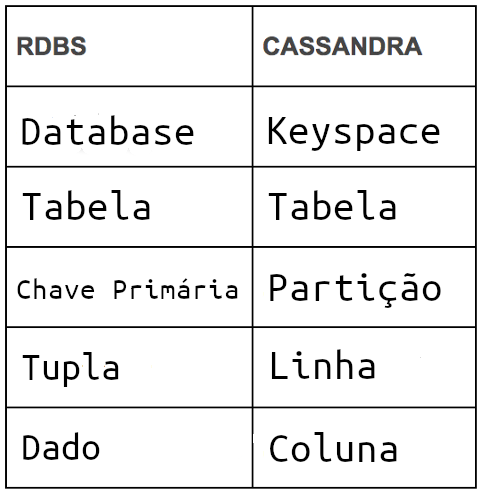
\includegraphics[width=0.3\textwidth]{imagens/comparativo}
	\caption{Comparativo entre Bancos SQL tradicionais (RDBS) e o Cassandra}
\end{figure}

Para conhecer mais comandos da CQL, podemos acessar o seguinte endereço: \url{https://cassandra.apache.org/doc/latest/}.